\pdfbookmark[1]{resonators}{resonators}
\chapter{Resonators}\label{chap:Electromagnetic waves}
    The coaxial cables are made of a conducting wire surrounded by an insulating layer which is then surrounded by a conducting shield \cite{Griffiths2018}. This gives a 1D transmission line with boundaries allowing only a monochromatic wave to pass \cite{Schuster2007}. An electromagnetic wave in a coaxial cable has as standard an impedance of 50 Ohm\cite{Griffiths2018}. The coaxial cable is connected to a feedline which is again capacitively coupled to some resonators. 
    \section{Transmission line resonator modeled as a LC circuit}
        \begin{figure} [h]
            \centering
                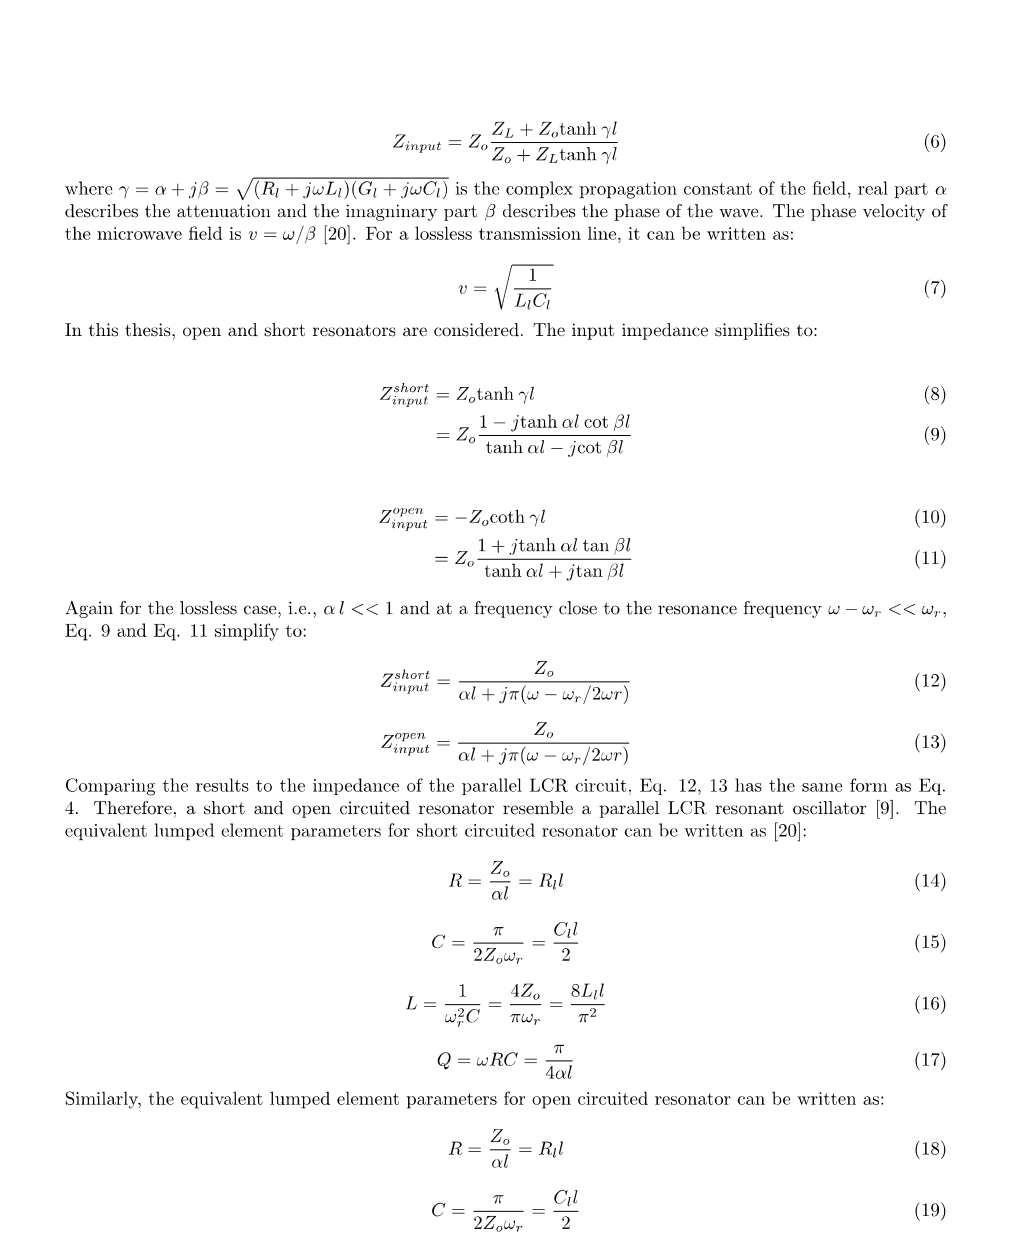
\includegraphics[width = 13cm]{Images/Transmission line resonator modeled as a LC circuit.png}
                \caption[Transmission line resonator modled as a LC Circuit]{\textbf{Transmission line resonator modled as a LC Circuit:} Here}
                \label{LC circuit}
        \end{figure}
    \section{Transmission line resonator capacitively coupled to}
        \begin{figure} [h]
            \centering
                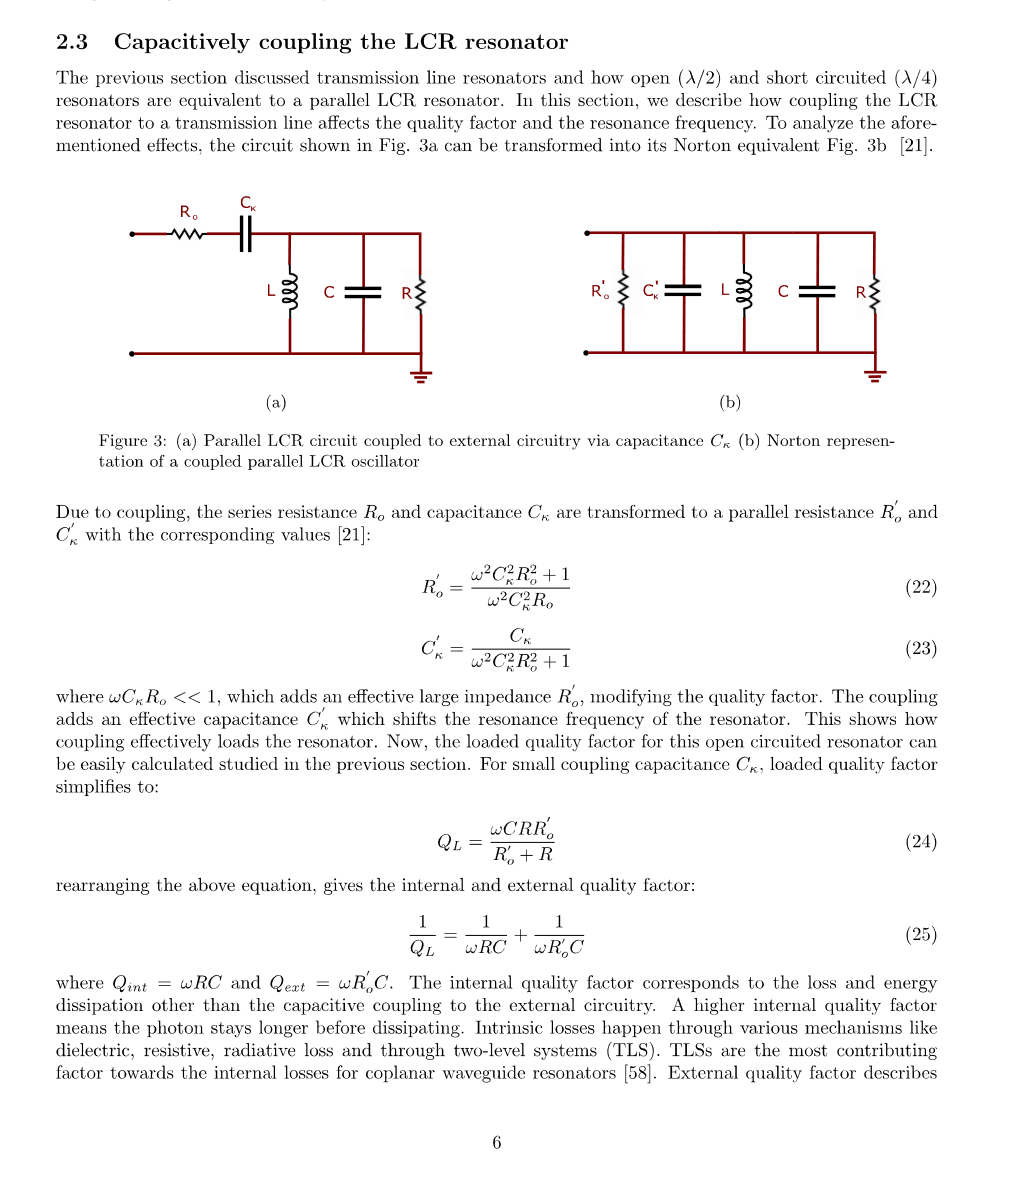
\includegraphics[width = 13cm]{Images/Transmission line resonator capacitively coupled to a feedline.png}
                \caption[Transmission line resonator capacitively coupled to a feedline]{\textbf{Transmission line resonator capacitively coupled to a feedline:} Here}
                \label{LC circuit capacitively coupled to feedline}
        \end{figure}
    Coplanar waveguide is a special type of transmission line resonators very commonly used in superconducting circuits for quantum building quantum computers (use some references here.) In the following section, we will describe what specifically type of coplanar waveguide (lambda 2 and lambda4 resonators (open and shunt)), how the electric field is distributed, how their geometry is, how they are described (mathematically), what materials are used and why (aluminium, because they are superconducting), 
    \section{Coplanar waveguide cavities modeled as LC circutis?}
    \begin{figure} [h]
        \centering
            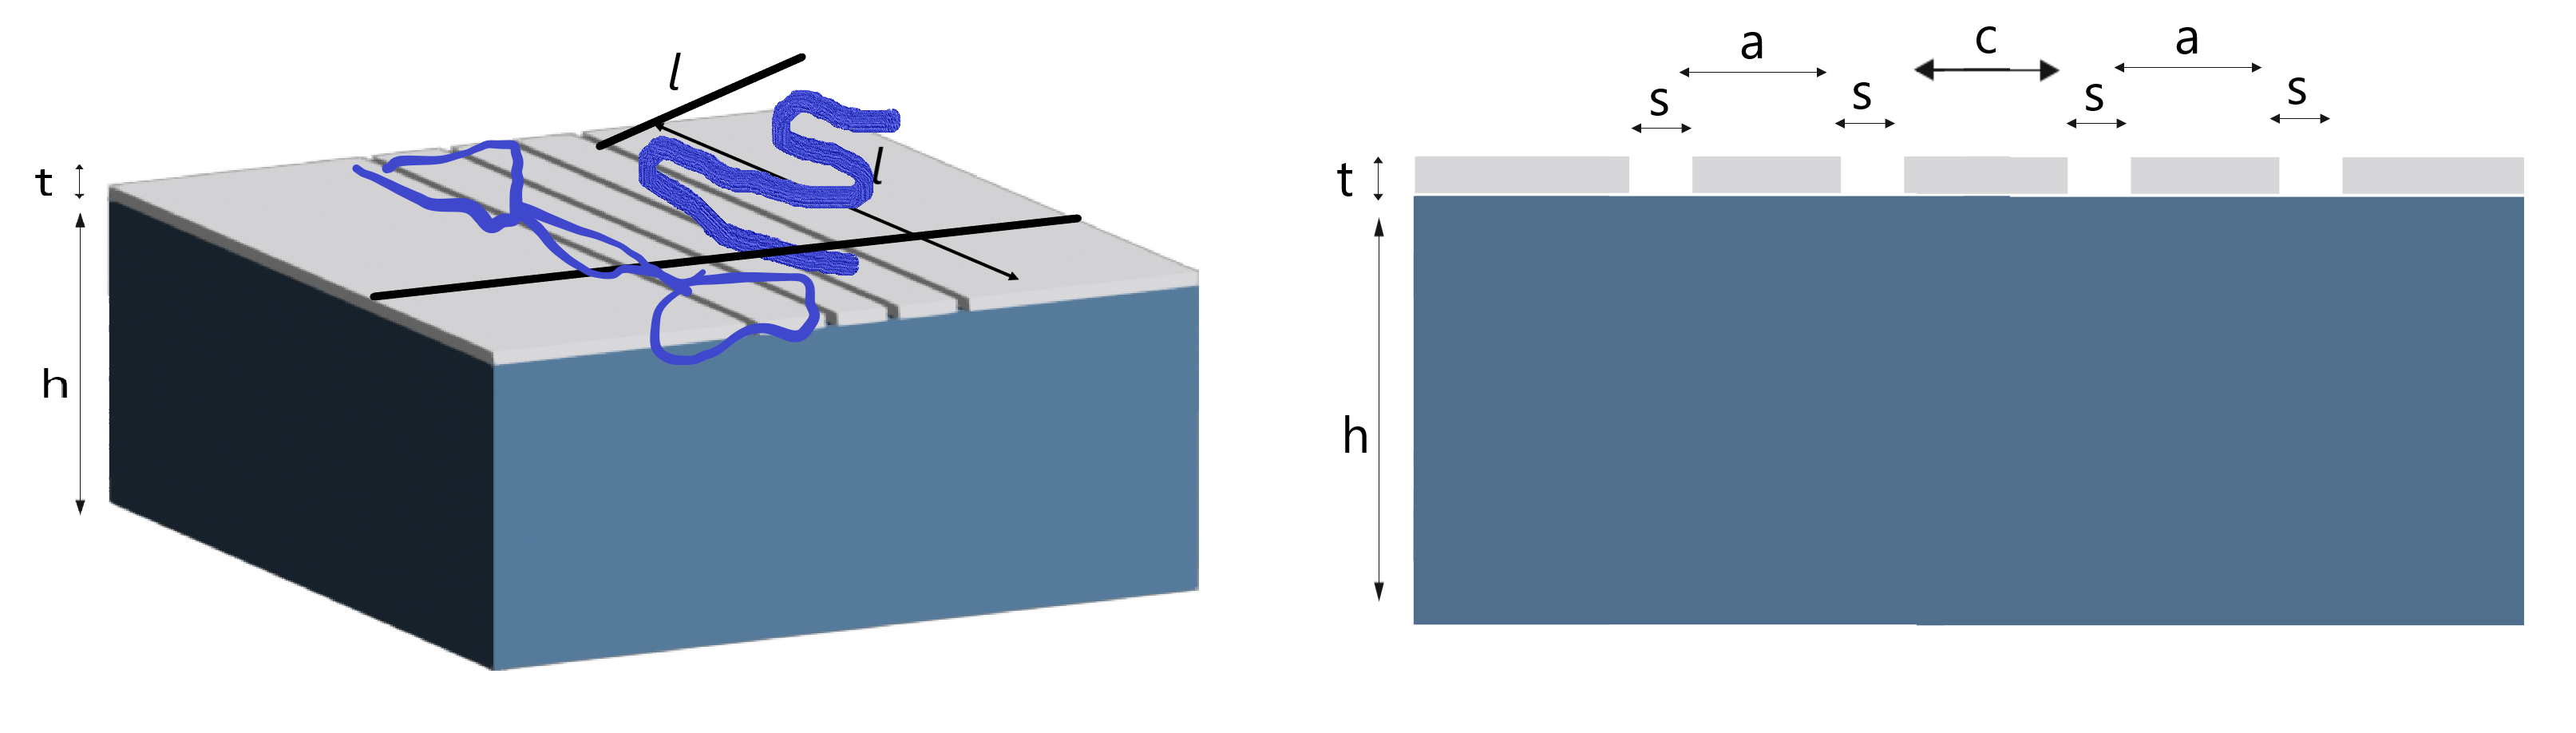
\includegraphics[width=13cm]{Images/2D_Chip_dim.png}
            \caption[Coplaner waveguide]{\textbf{Coplanar waveguide:} This is a model of a CPW feedline capacitively coupled to a CPW resonator. The left side is a picture of the top view of the whole chip. The right is a picture of the cross section taken at the black line found in the top view. The grey regions represents a superconducting film and the blue our substrate. The superconducting film is etched to create the resonators and the feedline. They both have width (a) and and distance (s) to the rest of the superconducting film for impedance matching.}
        \label{fig:2D_chip_dim}
    \end{figure}
    Feedlines and resonators have many similarities but are used very differently how??. While the feedline allow voltages and currents with many different magnitudes and phases to be transmitted through, the resonators only allows waves of specific frequencies to live inside it \cite{Pozar2012}. Fig. \ref{fig:2D_chip_dim} shows us the geometry of the feedline and the resonator. The left side is a top view of the whole chip containing a feedline and a resonator while the right side is a cross sectional view which highlight the device geometries. The cross section is taken at the black line shown in the top view. The grey regions represents a superconducting film and the blue our substrate. In this thesis, we will use Aluminium (Al) as our superconducting film and Silicon (Si) as our substrate. The superconducting film is etched to create the resonators and the feedline. They both have width (a) and and distance (s) to the rest of the superconducting film for impedance matching. 
    \newline
    \newline
    The device geometry and the dielectric properties of the resonators play a great role on the frequency. We are mainly working with $\lambda / 2$ and $\lambda / 4$ resonators \cite{Pozar2012}.  These two types of resonators can be engineered as a short- or open circuited as seen in fig. \ref{fig:lambda2_and_lambda4}. The frequency of the lambda and lambda4 resonator is given by \cite{Goppl2008}: 
    \begin{figure}
        \centering
            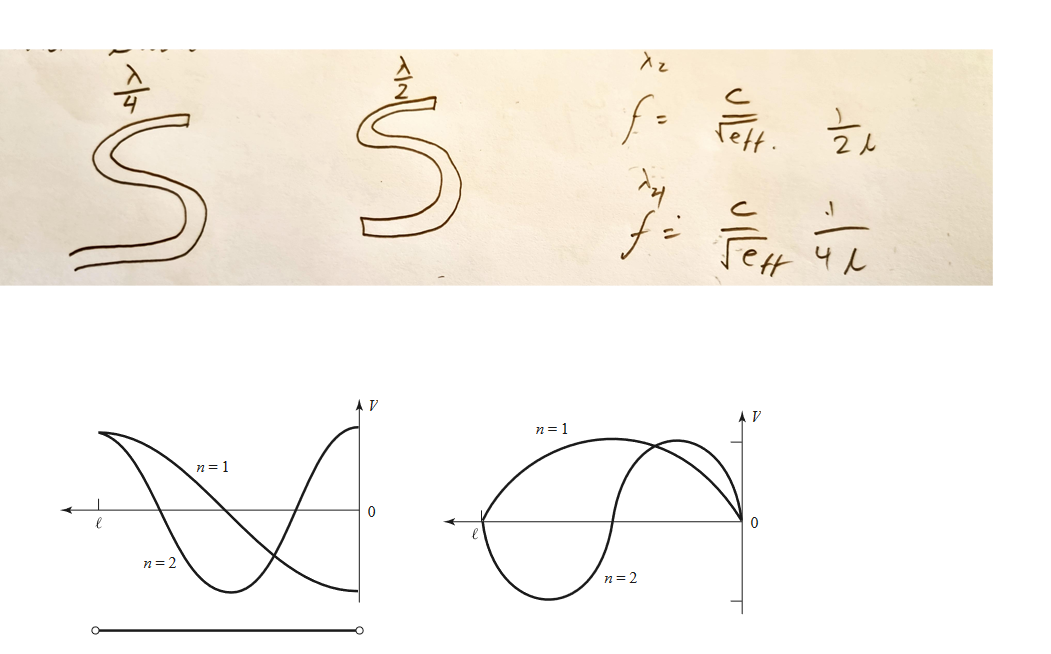
\includegraphics[width=10cm]{Images/lambda2 and lambda4 resonators_total.png}
            \caption[$\lambda$2 and $\lambda$4 resonators]{\textbf{$\lambda$2 and $\lambda$4 resonators:} This is a picture of the $\lambda$2 and $\lambda$4 resonators. The $\lambda$2 resonator are short in both ends.the $\lambda$4 has 1 end shorted and 1 end open}
        \label{fig:lambda2_and_lambda4}
    \end{figure}
    \begin{equation}
        \begin{aligned}
            w_{0,\lambda 2} &= \frac{c}{\sqrt{\epsilon_{\mathrm{eff}}}} \frac{1}{2 l} \\
            w_{0,\lambda 4} &= \frac{c}{\sqrt{\epsilon_{\mathrm{eff}}}} \frac{1}{4 l}
        \end{aligned}
    \end{equation}
    Where $2l = \lambda_{2,0}$ and $4l = \lambda_{4,0}$ is the wavelength of the resonator mode and the $\epsilon_{\mathrm{eff}}$ is the effective dielectric constant given by. 
    \begin{equation}
        \epsilon_{\mathrm{eff}}=\frac{1+\epsilon_{\mathrm{r}} \widetilde{K}}{1+\widetilde{K}}
    \end{equation}
    And K(k) and K(k') are elliptical integrals given by: 
    \begin{equation}
        \begin{gathered}
            \widetilde{K}=\frac{K\left(k^{\prime}\right) K\left(k_3\right)}{K(k) K\left(k_3^{\prime}\right)} \\
            k=\frac{a}{a+s} \\
            k_3=\frac{\tanh \left(\frac{\pi a}{4 h}\right)}{\tanh \left(\frac{\pi (a+s)}{4 h}\right)} \\
            k^{\prime}=\sqrt{1-k^2} \\
            k_3^{\prime}=\sqrt{1-k_3^2}
            \end{gathered}
    \end{equation}
	The frequency of both lambda4 and lambda2 resonators are highly dependent on the device geometry and the length of the resonators. Keeping the same geometries for all resonators in our system, we can vary their frequency by simply changing the length. 
    
    
    
    \subsection{Impedance}
        We can express the dissipation of our system as an impedance. At our typical operating temperature for superconducting systems ($T<T_c$) the DC resistance vanish shown by the meissner effect in the next section. However, there are a small non-zero contribution to the impedance due to the AC electric fields \cite{Zmuidzinas2012}. The impedance of the coaxial cable has to match the one of feedline and the resonator in order to eliminate as many unwanted reflections as possible as this will lead to power loss \cite{Pozar2012}. When the impedance matches perfectly, you will maximize the power transferred between each component. However, calculating impedance is strongly geometrical dependent. We can model both the feedline and the resonator as a LC lumped element.
        % Let's get something in the clear: 
        % \begin{itemize}
        %     \item $Z_{0}$ is the impedance from the the cables and is 50 ohms
        %     \item $Z_{r}$ = impedance inside the resonator?
        %     \item $Z_{fl}$ = impedance inside the feedline
        % \end{itemize}
        We always assume, that the impedance going from the cables to our system is $50 \Omega$ For a system which is in perfect impedance matching throughout the system, we use $Z_{0}$  for all of the values above. We can express the impedene of our resonators as \cite{Pozar2012}.
        \begin{equation}
            Z_{0} = \sqrt{\frac{L}{C}}
        \end{equation}
        Where L is the total inductance and C is the total capacitance of the resonator. 
        \begin{equation} 
            \begin{aligned}
                L &= \frac{2}{\pi^{2} n^{2}} L_{\ell} l \\
                C &=\frac{1}{2} C_{\ell} \ell
            \end{aligned}
        \end{equation}
        The $C_{\ell}$ is the capacitance (of what? the total capacitance or the capacitance of the coupling?) and depend on???
        It is given by the formula: 
        \begin{equation}
            C_{\ell}=4 \varepsilon_0 \varepsilon_{e f f} \frac{K(k)}{K\left(k^{\prime}\right)}
        \end{equation}
        l is the length of the resonator and $L_{l}$ is the total inductance. The inductance depend highly on the geometry and material properties at a certain temperature. It is given by 2 terms \cite{Schuster2007}:
        \begin{equation}
            \begin{gathered}
                L_m=\frac{\mu_0}{4} \frac{K\left(k^{\prime}\right)}{K(k)} \\
                L_k=\mu_0 \frac{\lambda_L^2}{W t} g(s, a, t) \\
                L_{\ell} = L_{m} + L_{k}
            \end{gathered}
        \end{equation}
        $L_m$ is the inductance stored in the feedline. The $L_k$ is the kinetic inductance and is due to the fact that electrons itself is creating a small inductance when moving \cite{Schuster2007}. $\mu_{0}$ is the Vacuum permeability and g is a geometrical function given by: 
        \begin{equation}
            g(s, a, t)=\frac{1}{2 k^2 K(k)^2}\left(-\ln \left(\frac{t}{4 a}\right)+\frac{2(a+s)}{(a+2 s)} \ln \left(\frac{s}{a+s}\right)-\frac{a}{(a+2 s)} \ln \left(\frac{t}{4(a+2 s)}\right)\right)
        \end{equation}
        Note that since our resonators has the geometry as a snake, there is also a contribution from the geometry in the inductance which is added, however this is not taken into account in this work. This shows, that the impedence is very sensitive to the device geometry. In order to match the impedance, we need to design the resonators and feedline to $ 50 \Omega$. 

    


        \subsection{Quality factors}
        The quality factor is a measure of how much energy is stored over how much energy is stored pr. time. We can use the Quality factor to say something about how lossy our circuit is in terms of photons. Many factors are at play when talking about the losses, conductor loss, dielectric loss, radiation loss. Often the losses occur due to the way of fabrication and there is no way to be sure what your $Q_factor$ are before fabrication. However, there are some equations relating the Q factor to the different components which are used for fitting the data later on. Systems like the one in fig. \ref{fig:2D_chip_dim} where a coplanar waveguide resoantor is capacitively coupled to a feedline, there are 2 characteristic qualitifactors to take into account. The intrinsic or unloaded quality factor, $Q_i$, and the external or the loaded quality factor, $Q_e$. The two quality factors have the following relation:
        \begin{equation}
            \frac{1}{Q_{T}} = \frac{1}{Q_{c}} + \frac{1}{Q_{i}} 
        \end{equation}
        The unloaded quality factor (that is how lossy the resonator is out of context in a coupled circuit), can be expressed by: 
        \begin{equation}
            Q_i=\omega_0 \frac{W_m+W_e}{P_{\text {loss }}}=\omega_0 R C=\frac{R}{\omega_0 L}
        \end{equation}
        The external quality factor highly depend on how strongly coupled the resonator is to the feedline and is described by: (FIND OUT WHAT THE x IS!)
        \begin{equation}
            \begin{aligned}
                Q_c &= \omega_0 C_T Z_x=\sqrt{\frac{C_T}{L}} \frac{2}{\omega_0^2 C_c^2 Z_0}\\    
            \end{aligned} 
        \end{equation}\label{eq:Qc}
        Even though the total capacitance is divided into two parts, we can find the total capacitance using the following relation: 
        \begin{equation}
            C_{T} = C + C_{c} = > C_{c} = C_{T} - C
        \end{equation}
        Where C is the unloaded resonator capacitance and $C_c$ is the capacitance due to coupling to the feedline. The coupling can be made smaller by making the gap larger (makes sense, but I  need to see it in the picture). 
        \\
        Depending on the fabrication and thereby the Q-factor, the electromagnetic wave will be scattered, transmitted and reflected with different ratios described by the scattering matrix: S



        \subsection{Looses in superconducting resonators}
        Many things can effect the quality factor. Since we can interpret the quality factor as a measure of how much dissipation there are inside the resonator, we typically say that "loss" in a superconducting resonator is the loss of photons. In the following we briefly mention some of the reasons for loss.
        \\
        Loss can occur as radiation into the free space \cite{Zmuidzinas2012}. 
        Losses are due to geometrical factors or defects occurring in the fabrication process. Why are we t in losses? changes the $Q_i$?
        \\
        Two level system loss
        \\	
        Magnetic vortices loss 
        \\
        Loss uncertainty 
        \\
        Radiation loss
        \\
        All these losses can lead to a change in the Q-factor and the scattering, transmission and reflection will also make our system non-ideal which results in transmission and  reflection and even phase change, amplitude changes and so on. 



    \subsection{Scattering Matrix}
        The scattering matrix give a description of how an incident wave is transmitted, reflected and scattered \cite{Pozar2012}. In this context, the matrix is used to relate the incident voltage wave with the reflected when using a 2 port network (from a VNA) connected to each end of the feedline. We are mostly interested in the transmission which takes the form \cite{Khalil2012}.  
        \begin{equation}
            S_{21} \equiv \frac{V_{out}}{V_{in}}
        \end{equation}
        Where $V_{in}$ is the voltage going into the feedline and $V_{out}$ is the voltage going out of the feedline. For a hanging resonator like the one in fig. \ref{fig:2D_chip_dim} this will give a dip like in fig. \ref{fig:resonator_dip}- 
        \begin{figure}[h]
            \centering
            \includegraphics[width = 10 cm]{Images/Resonator_dip.png}
            \caption[Characteristics of resonator dip]{\textbf{Characteristics of resonator dip:} This is a picture of how a resonator dip can look like.}
        \label{fig:resonator_dip}
        \end{figure}
        The transmitted voltage through the feedline can be fitted by a lorentzian taken the form \cite{Zmuidzinas2012}:
        \begin{equation}
            S_{21}(\omega) = 1 - \frac{\frac{Q_{l,r}}{Q_c}}{1+i2Q_{l,r}(\frac{\omega-\omega_0}{\omega_0})}
        \end{equation}
        Where $Q_{l,r}$ is the overall quality factor of the resonator, $Q_c$ is the coupling quality factor of the resonator and $\omega_0$ the resonator resonance frequency. This fitting model relates the Quality factors mentioned before and we use it to extract the $Q_i$ and $Q_c$ of our resonators. 
        % In order to focus on the central dip and not take the tail of the lorentzian into account, we find the full width at half maximum ($\delta_f$) which corresponds to around 3dB from the $S_{21}$ min  \cite{Barlow1989}.
        % \begin{equation}
        %     L = 10\cdot Log_{10}(\frac{P}{P_0}), \frac{P}{P_0} = 0.5 \Rightarrow L = 10\cdot Log_{10}(0.5) \approx 3 dB
        % \end{equation}
        % We will take this as the width of the dip. We can then express the relationship between the Q factors and the scattering matrix as:
        % Using this formula, we can write the unloaded Q_factor = Q_e as: 
        % \begin{equation}
        %     Q = \frac{\omega_0}{\Delta f}
        % \end{equation}
        \begin{equation}
            \begin{gathered}
                Q_c=\frac{Q_{l,r}}{1-\min \left(\left|S_{21}\right|\right)} \\
                Q_i=\frac{Q_{l,r}}{\min \left(\left|S_{21}\right|\right)}
            \end{gathered}
        \end{equation}
        Usually the $Q_c$ is close to the value found using the eq. \ref{eq:Qc} and is in the order of $e5$. You want as high $Q_i$ as possible we typically have in the order of  $e6$ but there have been shown $Q_i$ factors in the order of $e8$ for high powers \cite{Crowley2023b}. However, working with superconducting resonators, you typically want to see what your $Q_i$ is in the single photon regime as it is also the regime where we want to operate our qubit. In order to measure if we are in the single photon regime, we want to write a relation between the photon number and the power we send out. 


    \subsection{Photon number}
        We want to be in the single photon regime (in order to mimic the one of the qubit which is also just taking 1 photon in and 1 out). However, we can only estimate the number of photons \cite{Bruno2015}: 
        \begin{equation}
            \left\langle n_{p h}\right\rangle=\frac{2}{\hbar \omega_0^2} \frac{Q_{l,r}^2}{Q_c} P_{i n}
        \end{equation}
        Where $P_{in}$ is the number of photons going into the feedline and $\omega_0$ is the frequency of our resonator. We need to remember, that the current going from the VNA is the not the current going through our feedline as we have coupled a lot of different attenuators and amplifiers. These need to be taken into account. 
        

    \subsection{Quantization of the LC harmonic oscillator}
    From schuster p. 60. since we are working with QM, we want to describe the LC circuit quantum mechanically. The quantization gives a hamiltonian: 
    also blais p. 5
    \begin{equation}
        H = \hbar \omega (a^{\dagger} a + \frac{1}{2})
    \end{equation} 
    The energy of an inductor, the energy of a capacitor (as we should use it in the next section. )